


% Notes on style
%
% Identation
% Variable names
% Magic numbers, introducing final
%
%

\section{Introduction}
\label{sec:introduction}

Programs have lots of data, they are basically
ways of getting data, transforming data, and giving data back to the
world. 
%
Data types, as we have already seen, tell you which kinds of data you
have in your program. 

Computers store data in their memory in the form of bits. The word
``bit'' is a contraction of ``BInary digiT'', so a bit is
either~1~or~0, true or false, high or low, on or off. Bits are
organised in groups of 8 called \emph{bytes}. These bytes ---groups of
eight bits--- are used to store any data in the memory of the
computer. When you have got~1024~bytes, you have got a kilobyte or KB;
when you have~1024~KB you have got a megabyte or MB, and so on for
gigabytes~(GB), terabytes~(TB), and petabytes~(PB). Note that in
computing everything is measured in powers of~2 ($2^3 = 8, 2^{10} =
1024$) and not in powers of~10 as in normal life. That is because
computers count with bits~(2) and human beings\footnote{Not all humans
used only the ten fingers in their hands to count. Some languages like
French or Irish have remains of base-20 counting.} count with their
fingers~(10). 

\section{Simple data types}
\label{sec:simple-data-types}

Simple data types can be thought as boxes in the computer's
memory. Every time you declare a variable in your program, you can
think\footnote{This is only a metaphore and is not supposed to be an
  accurate description of how memory is managed on a modern
  computer. Explaining how things like the registers, the stack, and
  the heap work, the differences between actual machines and virtual
  machines, etc; are out of the scope of this document.} of the
computer as creating a little box in its memory to store your
variable. That box has two tags on it: one of them holds the name of
the variable and the other holds the type
(Figure~\ref{fig:github}). In the same way, you can think of
assignment as putting a value inside that box. 

\begin{figure}
  \centering
  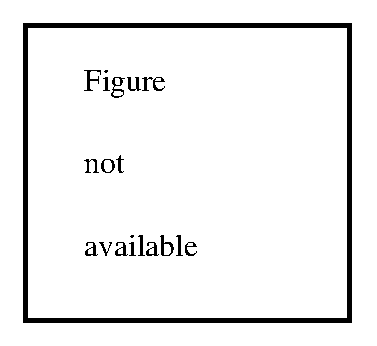
\includegraphics{gfx/no_figure}
  \caption{Declaring a variable in Groovy can be seen as creating a
    box. The box has a tag for the name and another for the type.}
  \label{fig:var1}
\end{figure}

\begin{figure}
  \centering
  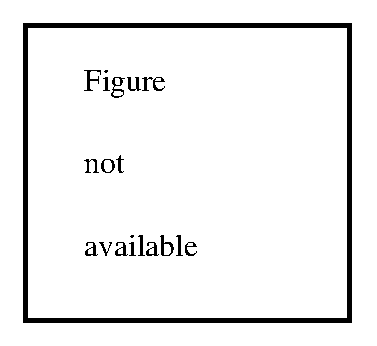
\includegraphics{gfx/no_figure}
  \caption{Assigning a value to a variable can be seen as putting a
    value in the box. If there was something in the box, it is
    overwritten and lost forever.}
  \label{fig:var2}
\end{figure}

\subsection{Static typing and dynamic typing}
\label{sec:strong-typing-weak}

You have already seen that Groovy, as most languages, puts some
restrictions to what you can use as a ``name'' tag for your boxes. You
know that they have to start with a letter: ``count'' is a valid name
but ``/me'' or ``5thNumber'' are not. You also know that some words
cannot be used by the programmer for variables names because it would
be confusing, e.g. ``while'', ``if'', ``System'', or ``println''.

Many programming languages also place one restriction on the ``type''
tag: once you decide the type of a variable, you cannot change
it. This is like people having static opinions that they do not want
to change. This type of languages are called \emph{statically typed
  languages} and, contrary to people with fixed ideas, they are
not necessarily bad or obnoxious. Java is an example of
statically typed language. 

Some programming languages allow you to change the type of your
variables as you go along, so you can have a variable that sometimes
is an int and later in time is a boolean or a String. These languages
are called \emph{dynamically typed languages}. They have pros and cons
compared to their statically typed counterparts. Groovy is an example
of a dynamically typed language. The following code excerpt is valid
in Groovy but not in Java. In Java a variable cannot be a String, and
then a boolean, and then a String again. Note that \emph{true} is a
boolean while \emph{``true''} (in quotes) is a String. 

\begin{verbatim}
    String str = "This is a string";
    str = true;   // This is different to: str = "true"
    if (str) {
      str = "This is a different string";
    }
\end{verbatim}

There are many more things to know about typing in programming
languages (strong vs. weak, inferred vs. manifest, duck typing, and
much more) but for now it will not be necessary to go into those
details. 

\subsection{Most common simple types}
\label{sec:most-common-simple}

\subsubsection{Integer numbers}
\label{sec:integers}

Integers (\verb+int+) are probably the most used simple data type, as
integer numbers are used for two of the most common operations in
computing: counting and indexing. Integers use~32~bits of memory, and
an integer variable can hold values between~-2,147,483,648 and
2,147,483,647~(inclusive). This data type is large enough for the
numbers needed in~90\%~of programs most people write. We have already
seen how to use it: 

\begin{verbatim}
    int count = 1
\end{verbatim}

There are two versions of integers for some special uses. When a
program needs very large (positive or negative) values, there is a
type \verb+long+, for \emph{long integer}. It is called ``long''
because it uses 64~bits instead of 32, which means a long integer
variable can hold values between -9,223,372,036,854,775,808 and
9,223,372,036,854,775,807 (inclusive). There is also a ``short''
integer that uses only 16~bits of memory (\verb+short+); this was
sometimes useful when Java was first released in 1995 but is hardly
ever used with modern computers. 

\subsubsection{Floating-point (decimal/rational) numbers}
\label{sec:float-point-decim}

Not all numbers are integer. Examples of common non-integer numbers
include the result of a division of two integers where one is not a
multiple of the other, and real-measurements like your height, your
weight, and the distance between your workplace and your home (unless
you work at home). In maths, these are called real numbers. In
computing they are usually called floating-point numbers and are
represented as a list of significant numbers and an exponent. The term
``floating-point'' refers to the fact that the decimal point can "float",
that is, it can be placed anywhere in the number changing the exponent
accordingly. 

$$ 1.23 \cdot 10^{-3} = 123 \cdot 10^{-5} = 0.00123 \cdot 10^0 $$

In Groovy and in Java, real numbers are usually represented with the
simple data type \verb+double+, that uses 64~bits. There is also a
32-bit version called \verb+float+ but, as with \verb+short+, it is
hardly used today.

\paragraph{Important note.} 

Floating-point numbers do \emph{not} have infinite precision, and
operating with them can cause rounding errors. There is a special type
for representing real values where precision is paramount (like in
banking): \verb+BigDecimal+. 

\subsubsection{Boolean (binary) values}
\label{sec:bool-binary-valu}

This simple data type represents one bit of information. It can hold
the values \verb+true+ and \verb+false+. 

\subsubsection{Characters}
\label{sec:characters}

Text is composed of characters: 'a', 'b', 'c'\ldots The \verb+char+ is
used to represent characters. It uses 16~bits, meaning it can
represent any of~65,536~different characters. 

Actually, the 16~bits of a char represent a Unicode symbol. Unicode is
a computing industry standard for the consistent encoding,
representation and handling of text expressed in most of the world's
writing systems. It includes symbols from most writing systems in
the world, including alphabets like Latin, Cyrillic, Arabic, or
Hebrew; syllabaries like Japanese katakana and hiragana, or
Cherokee; and many more. 

You may have noticed that we have not mentioned String yet. This is
because String is a complex type. 

\section{Complex types}
\label{sec:complex-types}

% Declaration and assignment... with "new"
% With capital letters



%%% Local Variables:
%%% mode: latex
%%% TeX-master: "main"
%%% End:
